\documentclass[11pt,a4paper]{article}

\usepackage[utf8]{inputenc}
\usepackage[T1]{fontenc}
\usepackage{lmodern}
\usepackage[english]{babel}
\usepackage{geometry}
\geometry{left=2.4cm,right=2.4cm,top=2.5cm,bottom=2.5cm}
\usepackage{graphicx}
\usepackage{xcolor}
\usepackage{hyperref}
\usepackage{booktabs}
\usepackage{longtable}
\usepackage{array}
\usepackage{enumitem}
\usepackage{listings}
\usepackage{float}
\usepackage{fancyhdr}
\usepackage{tikz}
\usepackage{amsmath}
\usepackage{parskip}

\usetikzlibrary{positioning}

\hypersetup{
    colorlinks=true,
    linkcolor=blue!60!black,
    urlcolor=blue!60!black,
    pdftitle={Developer Manual - Football Tournament Management System},
    pdfauthor={Rostand Cedrix Assonfo Demaboi}
}

\definecolor{codegray}{gray}{0.96}
\lstset{
    backgroundcolor=\color{codegray},
    basicstyle=\ttfamily\small,
    breaklines=true,
    frame=single,
    numbers=left,
    numberstyle=\tiny\color{gray},
    showstringspaces=false,
    tabsize=4,
    columns=fullflexible
}

\pagestyle{fancy}
\fancyhf{}
\lhead{Football Tournament Management System}
\rhead{Developer Manual}
\cfoot{\thepage}

\begin{document}

% ============================================================
% TITLE PAGE
% ============================================================

\begin{titlepage}
\centering
\vspace*{2cm}

{\Huge\bfseries Football Tournament Management System\par}
\vspace{0.8cm}
{\LARGE Developer Manual\par}

\vspace{1.5cm}
{\large Technical documentation based on the current source code\par}

\vspace{1.5cm}
\begin{tabular}{ll}
\textbf{Author:} & Rostand Cedrix Assonfo Demaboi \\
\textbf{Institution:} & Technische Hochschule Georg Agricola, Bochum \\
\textbf{Module:} & Introduction to Database Management Systems \\
\textbf{Semester:} & Summer Term 2026 \\
\textbf{Version:} & 1.0 \\
\end{tabular}

\vfill
{\large \today\par}
\end{titlepage}

\tableofcontents
\newpage

% ============================================================
\section{Purpose and Scope}

This document is the technical developer manual for the Football
Tournament Management System. It explains how the current repository
is structured, how the backend and frontend communicate, how the SQL
database is organized, how to run the application, and where a future
developer should modify the code when extending the system.

This manual is based on the source code contained in the submitted
project archive. Where the repository contains inconsistencies or
unfinished functionality, these points are explicitly identified.

\subsection{Functional Scope}

The application is intended to manage football competitions,
including:

\begin{itemize}
    \item tournaments;
    \item teams and coaches;
    \item players;
    \item scheduled matches;
    \item match scores;
    \item tournament rankings;
    \item organizer/viewer access concepts.
\end{itemize}

The SQL schema additionally contains users, player records, and the
many-to-many relationship between teams and tournaments.

% ============================================================
\section{Technology Stack}

\begin{longtable}{p{0.28\textwidth}p{0.62\textwidth}}
\toprule
\textbf{Component} & \textbf{Current implementation} \\
\midrule
Backend & Python, FastAPI, Uvicorn \\
Database access & SQLAlchemy ORM + psycopg2-binary \\
Database & PostgreSQL \\
Configuration & python-dotenv / environment variables \\
Frontend & Python Tkinter \\
HTTP client & Python requests \\
Containerization & Docker / Docker Compose \\
API documentation & FastAPI automatic documentation at \texttt{/docs} \\
Frontend packaging & \texttt{pyproject.toml} / uv configuration \\
\bottomrule
\end{longtable}

The backend currently declares:

\begin{lstlisting}
fastapi>=0.111.0
uvicorn>=0.29.0
psycopg2-binary>=2.9.0
python-dotenv>=1.0.0
\end{lstlisting}

The frontend requires Python 3.12 or newer and declares
\texttt{requests>=2.34.2}.

% ============================================================
\section{System Architecture}

The current application follows a client/server architecture.

\begin{figure}[H]
\centering
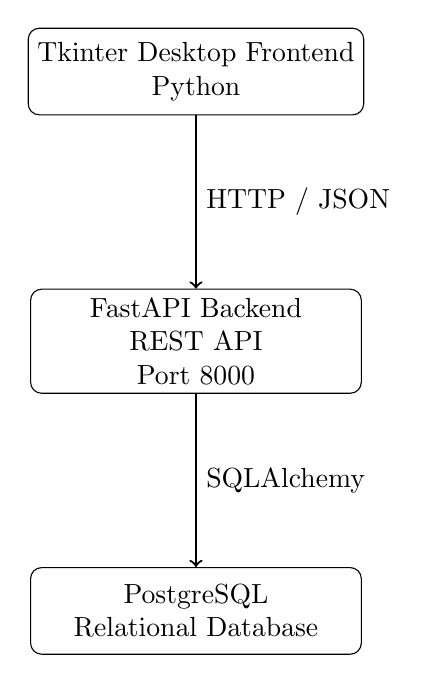
\begin{tikzpicture}[
    node distance=2.2cm,
    box/.style={
        rectangle,draw,rounded corners,
        minimum width=4.2cm,
        minimum height=1.1cm,
        align=center
    },
    arrow/.style={->,thick}
]
\node[box] (frontend) {Tkinter Desktop Frontend\\Python};
\node[box, below=of frontend] (backend) {FastAPI Backend\\REST API\\Port 8000};
\node[box, below=of backend] (database) {PostgreSQL\\Relational Database};

\draw[arrow] (frontend) -- node[right]{HTTP / JSON} (backend);
\draw[arrow] (backend) -- node[right]{SQLAlchemy} (database);
\end{tikzpicture}
\caption{Current application architecture}
\end{figure}

\subsection{Frontend Layer}

The frontend is located under:

\begin{lstlisting}
frontend/src/football_tournament/
\end{lstlisting}

It uses Tkinter and provides the connection screen, dashboard,
management forms and presentation of tournament data.

\subsection{Backend Layer}

The backend is located under:

\begin{lstlisting}
backend/app/
\end{lstlisting}

The FastAPI application is created in \texttt{main.py}. The current
application registers the following routers:

\begin{lstlisting}
/tournaments
/teams
/matches
\end{lstlisting}

\subsection{Database Layer}

The SQL database schema is defined in:

\begin{lstlisting}
database/init.sql
\end{lstlisting}

Test data is provided by:

\begin{lstlisting}
database/seed.sql
backend/seed.py
\end{lstlisting}

% ============================================================
\section{Repository Structure}

The relevant source structure is:

\begin{lstlisting}
football-tournament-manager/
|
+-- backend/
|   +-- app/
|   |   +-- models/
|   |   |   +-- __init__.py
|   |   +-- routes/
|   |   |   +-- tournaments.py
|   |   |   +-- teams.py
|   |   |   +-- matches.py
|   |   +-- schemas/
|   |   |   +-- __init__.py
|   |   +-- database.py
|   |   +-- auth.py
|   |   +-- main.py
|   +-- requirements.txt
|   +-- seed.py
|   +-- Dockerfile
|   +-- .env
|
+-- frontend/
|   +-- src/
|       +-- football_tournament/
|           +-- __main__.py
|           +-- api.py
|           +-- connection_dialog.py
|           +-- ui/
|               +-- dashboard.py
|   +-- pyproject.toml
|
+-- database/
|   +-- init.sql
|   +-- seed.sql
|
+-- docker-compose.yml
+-- README.md
\end{lstlisting}

\subsection{Backend Modules}

\begin{longtable}{p{0.38\textwidth}p{0.52\textwidth}}
\toprule
\textbf{Module} & \textbf{Responsibility} \\
\midrule
\texttt{app/main.py} & FastAPI application and router registration \\
\texttt{app/database.py} & SQLAlchemy engine, sessions and DB health check \\
\texttt{app/auth.py} & API token verification helper \\
\texttt{app/models/} & SQLAlchemy ORM models \\
\texttt{app/schemas/} & Pydantic schemas \\
\texttt{app/routes/tournaments.py} & Tournament operations \\
\texttt{app/routes/teams.py} & Team operations \\
\texttt{app/routes/matches.py} & Match operations \\
\texttt{seed.py} & Programmatic test-data insertion \\
\bottomrule
\end{longtable}

\subsection{Frontend Modules}

\begin{longtable}{p{0.42\textwidth}p{0.48\textwidth}}
\toprule
\textbf{Module} & \textbf{Responsibility} \\
\midrule
\texttt{api.py} & HTTP requests to the backend \\
\texttt{connection\_dialog.py} & Backend URL and token input \\
\texttt{ui/dashboard.py} & Dashboard and data display \\
\texttt{\_\_main\_\_.py} & Main application and management forms \\
\bottomrule
\end{longtable}

% ============================================================
\section{Database Design}

\subsection{Tables}

The SQL initialization script creates:

\begin{itemize}
    \item \texttt{users};
    \item \texttt{tournaments};
    \item \texttt{teams};
    \item \texttt{players};
    \item \texttt{matches};
    \item \texttt{team\_tournaments}.
\end{itemize}

\begin{figure}[H]
\centering
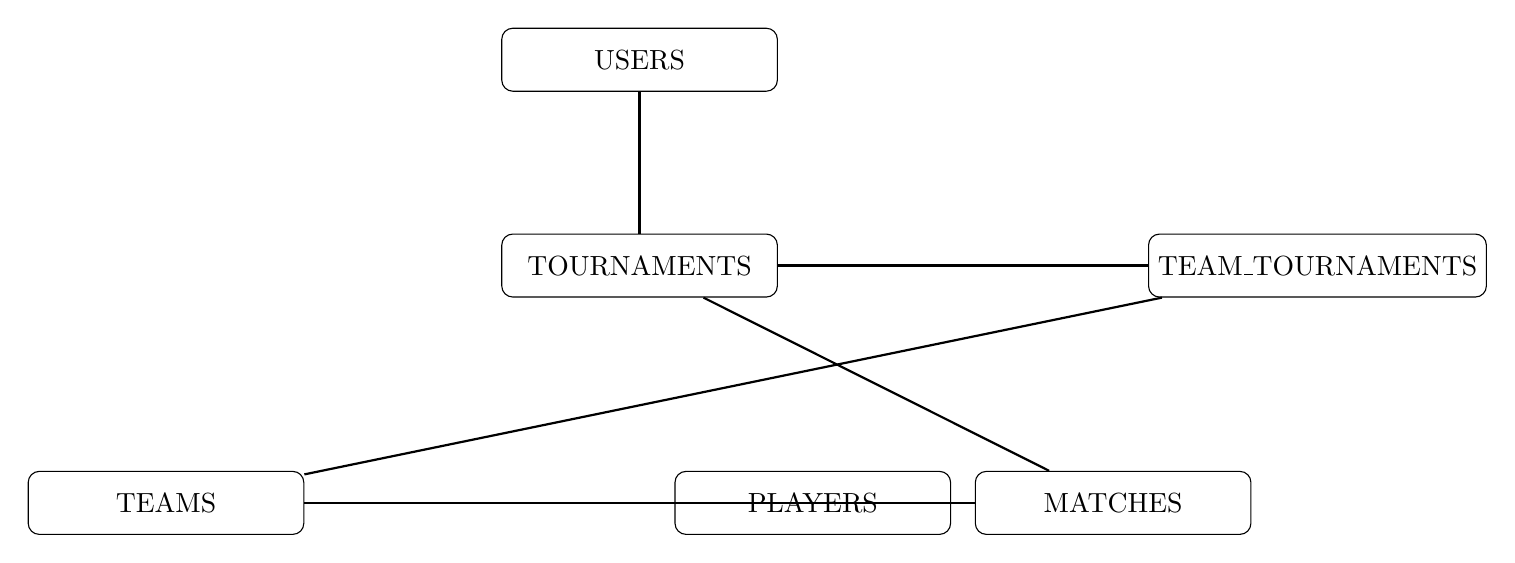
\begin{tikzpicture}[
    entity/.style={
        rectangle,draw,rounded corners,
        minimum width=3.5cm,
        minimum height=0.8cm,
        align=center
    }
]
\node[entity] (users) {USERS};
\node[entity, below=1.8cm of users] (tournaments) {TOURNAMENTS};
\node[entity, below left=2.2cm and 2.5cm of tournaments] (teams) {TEAMS};
\node[entity, below right=2.2cm and 2.5cm of tournaments] (matches) {MATCHES};
\node[entity, right=4.7cm of teams] (players) {PLAYERS};
\node[entity, right=4.7cm of tournaments] (tt) {TEAM\_TOURNAMENTS};

\draw[-,thick] (users) -- (tournaments);
\draw[-,thick] (tournaments) -- (matches);
\draw[-,thick] (teams) -- (matches);
\draw[-,thick] (teams) -- (players);
\draw[-,thick] (teams) -- (tt);
\draw[-,thick] (tournaments) -- (tt);
\end{tikzpicture}
\caption{Logical database relationships}
\end{figure}

\subsection{Users Table}

\begin{longtable}{llll}
\toprule
\textbf{Column} & \textbf{Type} & \textbf{Constraint} & \textbf{Meaning}\\
\midrule
user\_id & INTEGER & PK, Identity & User identifier\\
username & VARCHAR(50) & UNIQUE, NOT NULL & Username\\
email & VARCHAR(100) & UNIQUE, NOT NULL & Email\\
password & VARCHAR(255) & NOT NULL & Password/hash field\\
role & VARCHAR(20) & CHECK & organizer/player/viewer\\
created\_at & TIMESTAMP WITH TIME ZONE & DEFAULT & Creation time\\
\bottomrule
\end{longtable}

\subsection{Tournaments Table}

\begin{longtable}{llll}
\toprule
\textbf{Column} & \textbf{Type} & \textbf{Constraint} & \textbf{Meaning}\\
\midrule
tournament\_id & INTEGER & PK, Identity & Tournament identifier\\
name & VARCHAR(100) & NOT NULL & Tournament name\\
start\_date & DATE & NOT NULL & Start date\\
end\_date & DATE & NOT NULL & End date\\
organizer\_id & INTEGER & FK, NOT NULL & Organizer user\\
created\_at & TIMESTAMP WITH TIME ZONE & DEFAULT & Creation time\\
\bottomrule
\end{longtable}

The database enforces:

\begin{lstlisting}
CHECK (start_date <= end_date)
\end{lstlisting}

\subsection{Teams Table}

\begin{longtable}{llll}
\toprule
\textbf{Column} & \textbf{Type} & \textbf{Constraint} & \textbf{Meaning}\\
\midrule
team\_id & INTEGER & PK, Identity & Team identifier\\
name & VARCHAR(100) & UNIQUE, NOT NULL & Team name\\
coach & VARCHAR(100) & Nullable & Coach name\\
\bottomrule
\end{longtable}

\subsection{Players Table}

\begin{longtable}{llll}
\toprule
\textbf{Column} & \textbf{Type} & \textbf{Constraint} & \textbf{Meaning}\\
\midrule
player\_id & INTEGER & PK, Identity & Player identifier\\
first\_name & VARCHAR(50) & NOT NULL & First name\\
last\_name & VARCHAR(50) & NOT NULL & Last name\\
position & VARCHAR(30) & Nullable & Playing position\\
team\_id & INTEGER & FK, NOT NULL & Player team\\
\bottomrule
\end{longtable}

\subsection{Matches Table}

\begin{longtable}{llll}
\toprule
\textbf{Column} & \textbf{Type} & \textbf{Constraint} & \textbf{Meaning}\\
\midrule
match\_id & INTEGER & PK, Identity & Match identifier\\
match\_date & DATE & NOT NULL & Match date\\
home\_score & INTEGER & CHECK $\geq 0$ & Home score\\
away\_score & INTEGER & CHECK $\geq 0$ & Away score\\
tournament\_id & INTEGER & FK, NOT NULL & Tournament\\
home\_team\_id & INTEGER & FK, NOT NULL & Home team\\
away\_team\_id & INTEGER & FK, NOT NULL & Away team\\
created\_at & TIMESTAMP WITH TIME ZONE & DEFAULT & Creation time\\
\bottomrule
\end{longtable}

The schema also contains:

\begin{lstlisting}
CHECK (home_team_id != away_team_id)
\end{lstlisting}

\subsection{Team--Tournament Association}

\texttt{team\_tournaments} implements the many-to-many relationship
between teams and tournaments.

Its primary key is:

\begin{lstlisting}
PRIMARY KEY (team_id, tournament_id)
\end{lstlisting}

\subsection{Indexes}

The SQL initialization script creates indexes on tournament, home-team,
away-team, player-team and tournament-organizer foreign-key columns.

% ============================================================
\section{Backend Implementation}

\subsection{FastAPI Application}

The main FastAPI object is defined in
\texttt{backend/app/main.py}.

The application exposes:

\begin{lstlisting}
GET /
GET /health

/tournaments
/teams
/matches
\end{lstlisting}

\subsection{Database Access}

The database layer uses SQLAlchemy:

\begin{lstlisting}
engine = create_engine(DATABASE_URL)
SessionLocal = sessionmaker(
    autocommit=False,
    autoflush=False,
    bind=engine
)
\end{lstlisting}

Database sessions are provided to routes using the
\texttt{get\_db()} dependency.

\subsection{Tournament Routes}

The current implementation contains:

\begin{longtable}{llll}
\toprule
\textbf{Method} & \textbf{Path} & \textbf{Purpose}\\
\midrule
GET & /tournaments/ & List tournaments\\
GET & /tournaments/\{tournament\_id\} & Get one tournament\\
POST & /tournaments/ & Create tournament\\
DELETE & /tournaments/\{tournament\_id\} & Delete tournament\\
\bottomrule
\end{longtable}

\subsection{Team Routes}

\begin{longtable}{llll}
\toprule
\textbf{Method} & \textbf{Path} & \textbf{Purpose}\\
\midrule
GET & /teams/ & List teams\\
POST & /teams/ & Create team\\
DELETE & /teams/\{team\_id\} & Delete team\\
\bottomrule
\end{longtable}

\subsection{Match Routes}

\begin{longtable}{llll}
\toprule
\textbf{Method} & \textbf{Path} & \textbf{Purpose}\\
\midrule
GET & /matches/ & List matches\\
POST & /matches/ & Schedule a match\\
PUT & /matches/\{match\_id\}/score & Update score\\
DELETE & /matches/\{match\_id\} & Delete match\\
\bottomrule
\end{longtable}

\subsection{Health Check}

The endpoint:

\begin{lstlisting}
GET /health
\end{lstlisting}

returns the API status and the database connectivity status.

% ============================================================
\section{Pydantic Schemas}

The project defines Pydantic schemas for:

\begin{itemize}
    \item users;
    \item tournaments;
    \item teams;
    \item players;
    \item matches;
    \item team-tournament associations;
    \item ranking items;
    \item tournament rankings.
\end{itemize}

Important classes include:

\begin{lstlisting}
TournamentCreate
TeamCreate
PlayerCreate
MatchCreate
RankingItem
TournamentRanking
\end{lstlisting}

Not all schemas are currently connected directly to the route
functions. Some routes accept dictionaries or local Pydantic classes.

% ============================================================
\section{Authentication and Authorization}

The project contains an authentication helper in
\texttt{backend/app/auth.py}.

It expects:

\begin{lstlisting}
x-api-token: <token>
\end{lstlisting}

The expected token is read from the environment variable
\texttt{API\_TOKEN}, with a fallback value defined in the source.

The helper returns HTTP 401 for an invalid token.

\subsection{Current Integration Status}

The helper \texttt{verify\_token} exists, but the current route
registration does not attach it as a FastAPI dependency. Consequently,
the routes registered in \texttt{main.py} are currently not protected
by this helper.

A future developer should integrate the dependency before production
deployment.

% ============================================================
\section{Frontend Architecture}

\subsection{Startup}

The frontend entry point is:

\begin{lstlisting}
frontend/src/football_tournament/__main__.py
\end{lstlisting}

The application opens a connection screen and allows the user to
specify the backend URL and an optional token.

\subsection{Connection Dialog}

The default API URL is:

\begin{lstlisting}
http://localhost:8000
\end{lstlisting}

The current UI labels the token as \texttt{X-API-Token}.

\subsection{Dashboard}

The dashboard is implemented in:

\begin{lstlisting}
frontend/src/football_tournament/ui/dashboard.py
\end{lstlisting}

It contains four tabs:

\begin{itemize}
    \item Tournaments;
    \item Standings;
    \item Teams;
    \item Matches.
\end{itemize}

\subsection{Match Scheduling}

The scheduling form collects:

\begin{itemize}
    \item tournament;
    \item match date;
    \item home team;
    \item away team;
    \item referee.
\end{itemize}

The frontend prevents selecting the same team for both sides.

\subsection{Score Update}

The score form requires integer score values and calls:

\begin{lstlisting}
PUT /matches/{match_id}/score
\end{lstlisting}

% ============================================================
\section{Frontend API Client}

The API client is located at:

\begin{lstlisting}
frontend/src/football_tournament/api.py
\end{lstlisting}

It provides functions including:

\begin{lstlisting}
get_tournaments()
create_tournament(...)
get_teams()
create_team(...)
get_matches()
create_match_scheduled(...)
update_score(...)
get_standings(...)
\end{lstlisting}

The client sends the token through:

\begin{lstlisting}
x-api-token
\end{lstlisting}

% ============================================================
\section{Business Logic}

\subsection{Match Validation}

Both frontend and database validation prevent a team from playing
against itself.

\subsection{Score Validation}

The database requires non-negative scores:

\begin{lstlisting}
CHECK (home_score >= 0)
CHECK (away_score >= 0)
\end{lstlisting}

The frontend additionally checks that entered scores are numeric.

\subsection{Tournament Dates}

The database requires:

\begin{lstlisting}
CHECK (start_date <= end_date)
\end{lstlisting}

\subsection{Standings}

The ranking schema contains:

\begin{itemize}
    \item position;
    \item team name;
    \item matches played;
    \item goals scored;
    \item goals conceded;
    \item points.
\end{itemize}

The current backend route files do not implement the ranking endpoint
referenced by the frontend client. The ranking algorithm should
therefore be implemented and documented explicitly if standings are
intended to be a supported backend feature.

% ============================================================
\section{Running the Application}

\subsection{Docker}

The current \texttt{docker-compose.yml} defines a backend service
on port 8000.

Start it with:

\begin{lstlisting}[language=bash]
docker compose up --build -d
\end{lstlisting}

Check services:

\begin{lstlisting}[language=bash]
docker compose ps
\end{lstlisting}

View backend logs:

\begin{lstlisting}[language=bash]
docker compose logs backend
\end{lstlisting}

Stop services:

\begin{lstlisting}[language=bash]
docker compose down
\end{lstlisting}

\subsection{Backend Without Docker}

From the backend directory:

\begin{lstlisting}[language=bash]
pip install -r requirements.txt
uvicorn app.main:app --reload --host 0.0.0.0 --port 8000
\end{lstlisting}

\subsection{Frontend}

The frontend project requires Python 3.12 or newer.

A typical development command is:

\begin{lstlisting}[language=bash]
cd frontend
source .venv/bin/activate
python3 -m football_tournament
\end{lstlisting}

% ============================================================
\section{Database Initialization}

\subsection{SQL Initialization}

The schema is created by:

\begin{lstlisting}
database/init.sql
\end{lstlisting}

The script drops existing tables and recreates them in dependency order.

\subsection{Seed Data}

Test data is available in:

\begin{lstlisting}
database/seed.sql
\end{lstlisting}

The SQL seed creates users, one tournament, three teams, team
associations, six players and six matches.

\subsection{Python Seed Script}

The project also contains:

\begin{lstlisting}
backend/seed.py
\end{lstlisting}

This script creates tables using SQLAlchemy metadata and inserts
sample records.

The project therefore currently has two seed mechanisms. A future
developer should select one authoritative initialization strategy.

% ============================================================
\section{Development Workflow}

For a new feature, the recommended sequence is:

\begin{enumerate}
    \item Create a Git feature branch.
    \item Modify the SQL schema if necessary.
    \item Update SQLAlchemy models.
    \item Update Pydantic schemas.
    \item Implement backend business logic.
    \item Add or modify FastAPI routes.
    \item Update the frontend API client.
    \item Update the Tkinter interface.
    \item Add or update tests.
    \item Test the database constraints.
    \item Update the documentation.
\end{enumerate}

Example:

\begin{lstlisting}[language=bash]
git checkout -b feature/new-functionality

# Make changes

git add .
git commit -m "Add new functionality"
git push origin feature/new-functionality
\end{lstlisting}

% ============================================================
\section{Testing}

The inspected repository does not contain a dedicated automated
test suite.

A future test suite should cover:

\begin{itemize}
    \item database constraints;
    \item tournament operations;
    \item team operations;
    \item match scheduling;
    \item score updates;
    \item authentication;
    \item ranking calculation;
    \item API error handling.
\end{itemize}

A score-update test should verify that an existing match receives a
valid score, that the API returns success, and that the new values are
persisted in the database.

% ============================================================
\section{Known Issues and Technical Debt}
\label{sec:known-issues}

This section records inconsistencies found in the current repository.

\subsection{Docker Compose and PostgreSQL}

The README describes PostgreSQL as a Docker Compose service, but the
current \texttt{docker-compose.yml} defines only the backend service.
PostgreSQL must therefore either be provided externally or added to
Docker Compose.

\subsection{Database Configuration}

The submitted \texttt{backend/.env} defines individual variables such
as \texttt{DB\_HOST}, \texttt{DB\_NAME}, \texttt{DB\_USER},
\texttt{DB\_PASSWORD} and \texttt{DB\_PORT}.

However, \texttt{database.py} reads the single variable
\texttt{DATABASE\_URL}. These configurations are currently not aligned.

\subsection{Authentication Header}

The authentication helper and frontend use:

\begin{lstlisting}
x-api-token
\end{lstlisting}

while project documentation also refers to \texttt{X-API-Key}.
One convention should be selected and applied consistently.

\subsection{Authentication Dependency}

The \texttt{verify\_token} helper is not attached to the currently
registered routes. Authentication therefore exists in the codebase
but is not fully enforced by the current API routing configuration.

\subsection{Ranking Endpoint}

The frontend contains a function targeting:

\begin{lstlisting}
GET /tournaments/{tournament_id}/ranking
\end{lstlisting}

but the current tournament router does not implement this endpoint.

The dashboard also checks for a method named
\texttt{get\_tournament\_ranking}, whereas the API client defines
\texttt{get\_standings}. These interfaces should be unified.

\subsection{Duplicate API Client Function}

The frontend API module contains multiple definitions of
\texttt{create\_match\_scheduled}. Only the last definition is used by
Python. Duplicate definitions should be removed.

\subsection{Model and Route Naming}

The SQLAlchemy Team model defines \texttt{coach}, while the team route
contains compatibility logic for \texttt{coach\_name} and
\texttt{coach}. The application should use one canonical field name.

\subsection{Credentials}

The project archive contains a backend environment file with database
credentials. Secrets should not be committed to source control.
Production credentials should be rotated if they have been exposed.

% ============================================================
\section{How to Extend the Application}

A new data-driven feature should normally follow this flow:

\begin{figure}[H]
\centering
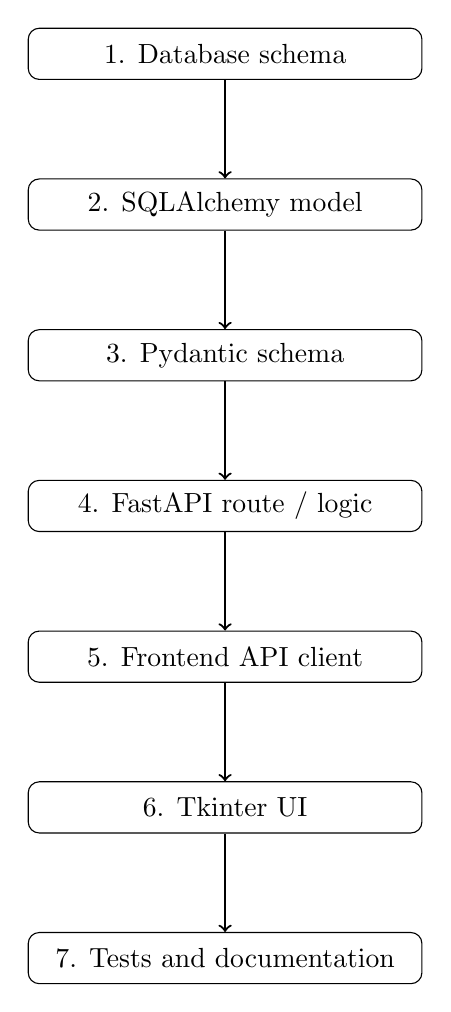
\begin{tikzpicture}[
    node distance=1.25cm,
    box/.style={
        rectangle,draw,rounded corners,
        minimum width=5cm,
        minimum height=0.65cm,
        align=center
    },
    arrow/.style={->,thick}
]
\node[box] (db) {1. Database schema};
\node[box, below=of db] (model) {2. SQLAlchemy model};
\node[box, below=of model] (schema) {3. Pydantic schema};
\node[box, below=of schema] (route) {4. FastAPI route / logic};
\node[box, below=of route] (api) {5. Frontend API client};
\node[box, below=of api] (ui) {6. Tkinter UI};
\node[box, below=of ui] (test) {7. Tests and documentation};

\draw[arrow] (db) -- (model);
\draw[arrow] (model) -- (schema);
\draw[arrow] (schema) -- (route);
\draw[arrow] (route) -- (api);
\draw[arrow] (api) -- (ui);
\draw[arrow] (ui) -- (test);
\end{tikzpicture}
\caption{Recommended feature implementation flow}
\end{figure}

For example, adding player management should update the database,
backend models and routes, frontend API client, interface and tests.

% ============================================================
\section{Maintenance Guidelines}

\begin{itemize}
    \item Keep SQL and SQLAlchemy models synchronized.
    \item Keep Pydantic schemas synchronized with API contracts.
    \item Do not commit secrets.
    \item Use environment variables for deployment-specific settings.
    \item Keep authentication header names consistent.
    \item Remove duplicate or obsolete frontend functions.
    \item Add tests when modifying business logic.
    \item Update this manual when the architecture changes.
\end{itemize}

% ============================================================
\section{Appendix: Useful Commands}

\begin{longtable}{p{0.55\textwidth}p{0.35\textwidth}}
\toprule
\textbf{Command} & \textbf{Purpose}\\
\midrule
\texttt{docker compose up --build -d} & Build and start services\\
\texttt{docker compose ps} & Display service status\\
\texttt{docker compose logs backend} & Display backend logs\\
\texttt{docker compose down} & Stop Docker services\\
\texttt{uvicorn app.main:app --reload} & Run FastAPI in development\\
\texttt{python3 -m football\_tournament} & Start Tkinter frontend\\
\bottomrule
\end{longtable}

\subsection{FastAPI Documentation}

When the backend is running, the interactive documentation is normally
available at:

\begin{lstlisting}
http://localhost:8000/docs
\end{lstlisting}

The OpenAPI schema is available at:

\begin{lstlisting}
http://localhost:8000/openapi.json
\end{lstlisting}

\end{document}
